\begin{figure}
  \ContinuedFloat*
  \begin{tabular}[t]{c c}
    \begin{minipage}{0.5\textwidth}
      \begin{Verbatim}[mathescape,commandchars=\\\{\}]
\textbf{let} s = stim 2 \textbf{in}
  \textbf{let} p = pop 2 \textbf{in}
      $\otimes$ s p 1
      \end{Verbatim}
    \end{minipage} & \begin{minipage}{0.5\textwidth}
      \includegraphics[width=\textwidth]{chapters/volr/example2.pdf}
    \end{minipage}

  \end{tabular}
  \caption{A textual and visual example of a network
    with a stimulus containing two channels. 
    The stimulus is fully connected to a population with an excitatory
    weight of 1. Each node represents a single neuron.}
  \label{fig:volr-example1}
\end{figure}

\begin{figure}
  \ContinuedFloat
  \begin{tabular}[t]{c c}
    \begin{minipage}{0.5\textwidth}
      \begin{Verbatim}[mathescape,commandchars=\\\{\}]
\textbf{let} s1 = stim 1 \textbf{in}
  \textbf{let} s2 = stim 1 \textbf{in}
    \textbf{let} p = pop 1 \textbf{in}
      $\ominus$ s1 p 1
      $\ominus$ s2 p -1
      \end{Verbatim}
    \end{minipage} & \begin{minipage}{0.5\textwidth}
      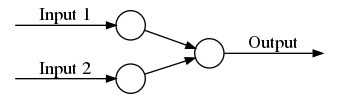
\includegraphics[width=\textwidth]{chapters/volr/example1.pdf}
    \end{minipage}
  \end{tabular}
  \caption{An illustration of a simple network that can solve a simple
    T-maze task. A single population (\texttt{\textbf{p}}) is 
    excited and inhibited by two different stimulus channels.
    The weights are initialised to the value of 1.}
  \label{fig:volr-example2}
\end{figure}

\begin{figure}
  \ContinuedFloat
  \begin{tabular}[t]{c c}
    \begin{minipage}{0.4\textwidth}
      \begin{Verbatim}[mathescape,commandchars=\\\{\}]
\textbf{let} s = stim 256 \textbf{in}
  \textbf{let} p = pop 256 \textbf{in}
    \textbf{let} o = pop 10 \textbf{in}
      $\ominus$ s p 1
      $\otimes$ p o 1
      \end{Verbatim}
    \end{minipage} & \begin{minipage}{0.6\textwidth}
      \includegraphics[width=\textwidth]{chapters/volr/example3.pdf}
    \end{minipage}
  \end{tabular}
  \caption{A more advanced example where the nodes are no longer single
    neurons, but populations of neurons. 
    This network can process the MNIST dataset as 16x16 images and
    infer the displayed number. Here the input is connected one-to-one
    with the first population (256), which is connected all-to-all to the 
    output population (9).}
  \label{fig:volr-example2}
\end{figure}